Para comenzar con el diseño de la aplicación y tras conocer el dominio de esta, se procede a realizar el mapa de navegación, el cual se puede observar en la \textbf{Figura \ref{fig: Mapa_navegacion}}. Este mampa consiste en una representación resumida del sitio web que además permite especificar las ``pulsaciones'' que un usuario debe realizar para que alcance una vista en específico.

\begin{figure}[h!tb]
    \hspace{-9mm}
    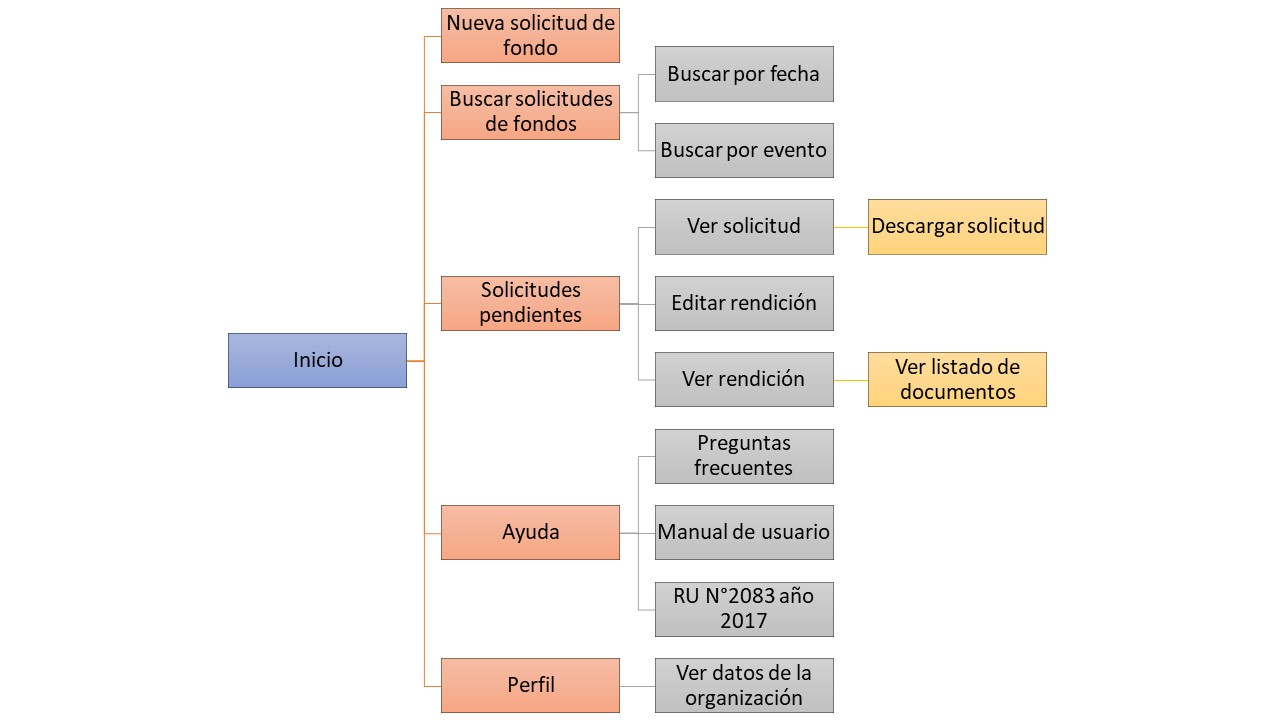
\includegraphics[width=1.1\textwidth]{Imagenes/Mapa_de_navegacion.jpg}
    \caption{\label{fig: Mapa_navegacion}Mapa de navegación de la aplicación.}
\end{figure}

A continuación se describen las principales vistas que tiene la aplicación:

\paragraph{Buscar solicitudes de fondos: }vista que ayuda al usuario a realizar busqueda de solicitudes realizadas a través del nombre del evento o por fechas.

\paragraph{Nueva solicitud de fondo: }vista que ayuda al usuario a inicializar un proceso de fondo por rendir. En esta fase se realiza la solicitud del evento con toda la información requerida y va dirigida a la Dirección de Escuela o DAAE según sea el caso (ver \textbf{Sección \ref{sec:Conceptos}}).

\paragraph{Solicitudes pendientes: }vista ayuda al usuario al rápido acceso de solicitudes que no están finalizadas. Dependiendo del estado en que se encuentre el fondo por rendir es lo que podrá acceder el usuario. Por ejemplo, si la Solicitud no ha sido aprobada y no se ingresa los datos de la RU que corresponde a la Solicitud, no se puede acceder a realizar la rendición del evento.

\paragraph{Ayuda: }vista en donde se encuentra toda la documentación que requiere el usuario para realizar un proceso de fondos por rendir.

\paragraph{Perfil: }vista que muestra toda la información correspondiente a una OE junto con los datos de la Dirección encargada de la validación de solicitudes y rendiciones de un evento antes de ser enviada a funcionarios superiores.